%%%%%%%%%%%%%%%%%%%%%%%%%%%%%%
%
%		Master thesis proposal
% 	Visualisation of Gene Ontology and Cluster Analysis Results
%	Author: Vladyslav Aleksakhin

\documentclass[a4paper,oneside]{article}

\usepackage{tabularx}
\usepackage{graphicx}
\usepackage{url}
\usepackage{color}
\usepackage{listings}


\newcommand*{\mywebref}[3]{
	\bibitem{#1} #2 is available on the web \url{#3}. Last access in September 2010.
}

\newcommand*{\todo}[1]{
	\begin{LARGE}
		\textcolor{red}{#1}
	\end{LARGE}
}
 
\begin{document}

\begin{titlepage}
\begin{center}

\Huge{Visualisation of Gene Ontology and Cluster Analysis Results}

\vfill

\begin{Large}
Master's Thesis Report (30 credit points)

\vfill

Superviser: Prof. Dr. Andreas Kerren\\
Student: Vladyslav Aleksakhin

\vfill

Linneuniversitetet\\
School of Mathematics and System Engineering

\end{Large}


\end{center}
\end{titlepage}

\tableofcontents
\newpage

\section{Abstract}

\newpage

\section{Abstract}

\section{Acknowledgments}

\section{Introduction}

\subsection{Bioinformatic}

\subsection{Information Visualization}

\subsection{Gene Ontology}

\subsection{Clustering}

\section{Problem Statements and Goals}

\subsection{Problem Statement}

\subsection{Dataset description}
Gene Ontology data and cluster analysis results presented as directed graphs. They are stored in separate files in special format -- GML files. GML file format covered in the next section.


GO graph is directed acyclic graph has 10042 verticies and  24155 edges. It has 1 root, 2729 nodes and 7312 leafs (terminal nodes).


Cluster graph is directed binary  tree has 14623 nodes and 14622. Cluster graph as a tree has 1 root, 7310 nodes and 7312 leafs.


Both of two graphs are independent from each other from developer point of view: they have different node ids and edge ids. But they are corresponded by graph node labels -- both of this graphs have same label for terminal graph nodes. This property is used in the subgraph extracting algorithm. 

\todo{add connections between graphs}

\subsection{GML}
 "GML, the Graph Modelling Language, is our proposal for a portable file format for graphs. GML's key features are portability, simple syntax, extensibility and flexibility. A GML file consists of a hierarchical key-value lists. Graphs can be annotated with arbitrary data structures. The idea for a common file format was born at the GD'95; this proposal is the outcome of many discussions. GML is the standard file format in the Graphlet~cite{Graphlet} graph editor system. It has been overtaken and adapted by several other systems for drawing graphs."~\cite{GML}
 
 
GML format is platform independent, and easy to implement. Furthermore, it has the capability to represent arbitrary data structures, since advanced programs have the need to attach their specific data to nodes and edges. GML is flexible enough that a specific order of declarations is not needed, and that any non-essential data may be omitted. Simple graph is showed in the Listing~\ref{sample_graph_gml}


\begin{center}
	\lstinputlisting[language=xml, tabsize=2, caption={GML description of sample graph}, label={sample_graph_gml}]{SampleGraph.gml}
\end{center}


In the Figure~\ref{sample_graph_yed_vis} showed manual visualization of the graph using yEd~\cite{yEd}


\begin{center}
\begin{figure}
	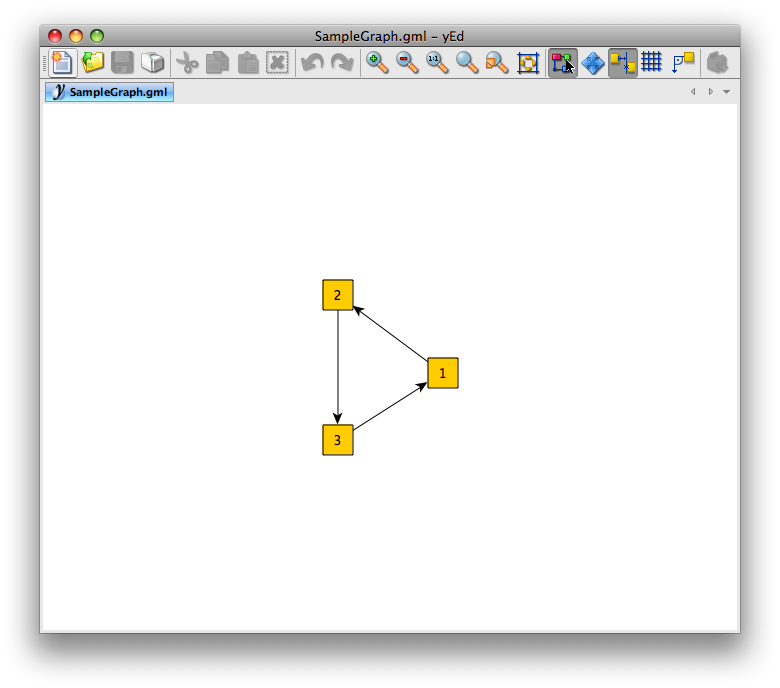
\includegraphics[scale=0.5]{SampleGraph.png}
	\caption{Manual visualization of the sample graph}
	\label{sample_graph_yed_vis}
\end{figure}
\end{center}


More complex graph with additional properties and its visualization produced by yEd graph editor is in the Listing~\ref{yed_graph} and showed on the Figure~\ref{yed_graph_vis}


\begin{center}
	\lstinputlisting[language=xml, tabsize=2, caption={GML graph with additional properties}, label={yed_graph}]{YedGraph.gml}
\end{center}


\begin{center}
\begin{figure}
	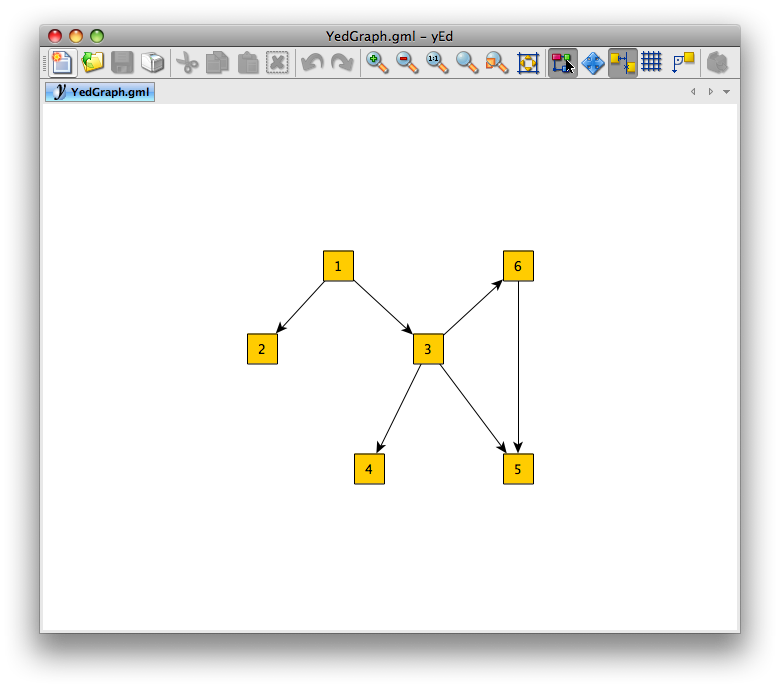
\includegraphics[scale=0.5]{YedGraph.png}
	\caption{Manual visualization of the sample graph}
	\label{yed_graph_vis}
\end{figure}
\end{center}


Applications supporting GML~\cite{GML_wiki}

\begin{enumerate}
\item Clairlib~\cite{clairlib}, a suite of open-source Perl modules intended to simplify a number of generic tasks in natural language processing (NLP), information retrieval (IR), and network analysis (NA).
\item Cytoscape~\cite{Cytoscape}, an open source bioinformatics software platform for visualizing molecular interaction networks, loads and save previously-constructed interaction networks in GML.
\item NetworkX~\cite{NetworkX}, an open source Python library for studying complex graphs.
\item ocamlgraph\cite{ocamlgraph}, a graph library for OCaml.
\item OGDF\cite{OGDF}, the Open Graph Drawing Framework, an open source C++ library containing implementations of various graph drawing algorithms. The library is self contained; optionally, additional packages like LP-solvers are required for some implementations.
\item Tulip~\cite{Tulip} (software) is a free software in the domain of information visualisation capable of manipulating huge graphs (with more than 1.000.000 elements).
\item yEd~\cite{yEd}, a free Java-based graph editor, supports import from and export to GML.
\end{enumerate}

\section{Solution}

\subsection{Cluster Analysis Results Visualization}

\subsection{Gene Ontology Visualization}

\section{Implementation}
\subsection{IO layer}
\subsection{Gene Ontology Visualization Implementation}
\subsection{Cluster Visualization Implementation}
	
\section{Conclusions}
\section{Results}

\section{Glossary}
GO -- Gene Ontology\\
XML -- eXtensible Markup Language
GML -- Graph Modelling Language

\begin{thebibliography}{99}

\mywebref{Biology}{Biotech}{biotech.icmb.utexas.edu/pages/bioinfo.html}

\mywebref{Bioinformatic}{Information about Bioinformatics}{www.absoluteastronomy.com/topics/Bioinformatics}

\mywebref{GO_website}{Gene Ontology}{www.geneontology.org/}

\mywebref{OBO}{The Open Biomedical Ontologies}{www.obofoundry.org/}

\mywebref{IPK}{Network Analysis Group (at IPK)}{nwg.bic-gh.de/}

\mywebref{Graphlet}{Graphlet}{http://www.fmi.uni-passau.de/Graphlet/}

\mywebref{GML}{GML}{http://www.infosun.fim.uni-passau.de/Graphlet/GML/gml-tr.html}

\mywebref{GML_wiki}{GML supported programs}{http://en.wikipedia.org/wiki/Graph_Modelling_Language}

\mywebref{yEd}{yEd}{http://www.yworks.com/en/products_yed_about.html}
\mywebref{clairlib}{Clairlib}{http://www.clairlib.org/}
\mywebref{Cytoscape}{Cytoscape}{http://en.wikipedia.org/wiki/Cytoscape}
\mywebref{NetworkX}{NetworkX}{http://en.wikipedia.org/wiki/NetworkX}
\mywebref{ocamlgraph}{ocamlgraph}{http://ocamlgraph.lri.fr/}
\mywebref{OGDF}{OGDF}{http://www.ogdf.net/}
\mywebref{Tulip}{Tulip}{http://tulip.labri.fr/TulipDrupal/}


\mywebref{GDC}{Graph Drawing Conference '95}{www.informatik.uni-trier.de/~ley/db/conf/gd/gd95.html}

\mywebref{Radial_dendrogram}{Radial Dendrogram}{cs.sunysb.edu/~vislab/papers}

\mywebref{Dendrogram}{Introduction into Dengrograms}{en.wikipedia.org/wiki/Dendrogram}

\bibitem{Barlow_Neville}
T. Barlow and P. Neville, A comparison of 2D visualization of hierarchies, Information Visualization pp 131-138, 2001.

\bibitem{Kreussler_Schumann}
M. Kreussler and H. Schumann, A flexible approach for visual data mining, IEEE Trans. VisualGraphics, vol. 8, no. 1, pp. 39-51, 2002.

\bibitem{Yang_Ward}
J. Yang, M. Ward, and E. Rundensteiner, InterRing: An interactive tool for visually navigating and manipulatiung hierarchical structures, IEEE 2002 Symposium on Information Visualization, pp. 77-92, 2002.

\mywebref{GEF}{Java Graph Editing Framework}{gef.tigris.org/}

\mywebref{ILOG_Jview}{ILOG Jview}{www.ilog.com/products/jviews/}

\mywebref{JUNG}{Java Universal Network / Graph Framework (JUNG)}{jung.sourceforge.net/}

\mywebref{JGraphT}{JGraphT)}{jgrapht.sourceforge.net/}

\mywebref{Piccolo}{Piccolo)}{www.cs.umd.edu/hcil/jazz/}

\mywebref{VTK}{Visualisation Toolkit)}{www.vtk.org/}

\mywebref{InfoVis_Toolkit}{InfoVis Toolkit)}{ivtk.sourceforge.net/}

\mywebref{Improvise}{Improvise project homepage}{www.cs.ou.edu/~weaver/improvise/index.html}

\end{thebibliography}

\end{document}